\documentclass[../document.tex]{subfiles}
\begin{document}
\section{Quarry dataset}
\label{sec: quarry-dataset}
After showing the model's capability of correctly separate classes' features we utilized Grad-CAM to visualize some of the samples in the test set. We divided those inputs in four classes based on the model's performance: worst, best, false positive and folse negative. We expect the worst and the best output to be on the left and the right branch of figure \ref{fig: pca-test-patches} respectively, while the other two categories to be in the mixed points.
We randomly sampled twenty inputs from those set and appplied Grad-CAM as texture on the 3D render to better visualize which region of the inputs caused the prediction. 
% \subsection{Best}
% We start evaluating our model by using the test set composed by samples from the Quarry map. We expect the model to correctly classify the patches with easy to see features such as big obstacles, steep ramps and holes. Unfortunately, the dataset is not trivial and most of the patches are challenging to classify even to human eye. 

% For instance, if look at patches, for some of them is not so easy to estimate the advancement by human eye. This is due to the specific robot locomotion that depends on the starting pose. Our goal in this section is to explain the model predictions on different inputs. 

\subsection{Best}
Best patches have few obstacles. We can obsverse two main clusters of images, flat and slopes. Interesting, when a surface has uneven ground near the left part, so close the the rear legs of the robot, the model is more interesting in those spots, \ref{fig : quarry-best-0}, \ref{fig : quarry-best-2}, \ref{fig : quarry-best-3}, \ref{fig : quarry-best-4}, \ref{fig : quarry-best-15}, \ref{fig : quarry-best-16}, \ref{fig : quarry-best-17}, \ref{fig : quarry-best-18}. This an expected behaviour since if there is an obstacle near the rear legs, then the robot will not be able to advance since it will be stuck from the beginning. 

Moreover, in other patches \ref{fig : quarry-best-1},  \ref{fig : quarry-best-8},  \ref{fig : quarry-best-9},  \ref{fig : quarry-best-19}, the model's also looks ahead of the robot. In those situation the robot is able to properly move at the beginning so the network must evaluate the possibility of obstacles ahead. There are two oblious cases, \ref{fig : quarry-best-8} and  \ref{fig : quarry-best-19}. The first one is a totally flat surface, so the model will look as far as possible to the robot's position to check if there are obstacles. Simarly, in the second, a surface with a bump in the hend, the network controls that spot. So, correctly, the network analysis the first region of the patch that may contain an untraversable obstacle.
\begin{figure}[H]
    \centering
    \begin{subfigure}[b]{0.192\linewidth}
    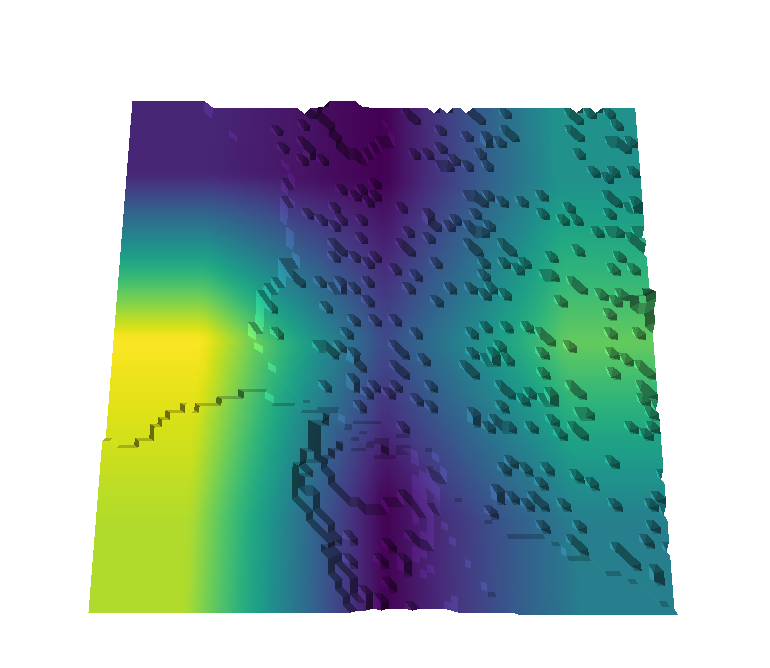
\includegraphics[width=\linewidth]{../img/5/quarry/best/20-patch-3d-majavi-colormap-0.png}
    \caption{0.20cm}
    \label{fig : quarry-best-0}
    \end{subfigure}
    \begin{subfigure}[b]{0.192\linewidth}
    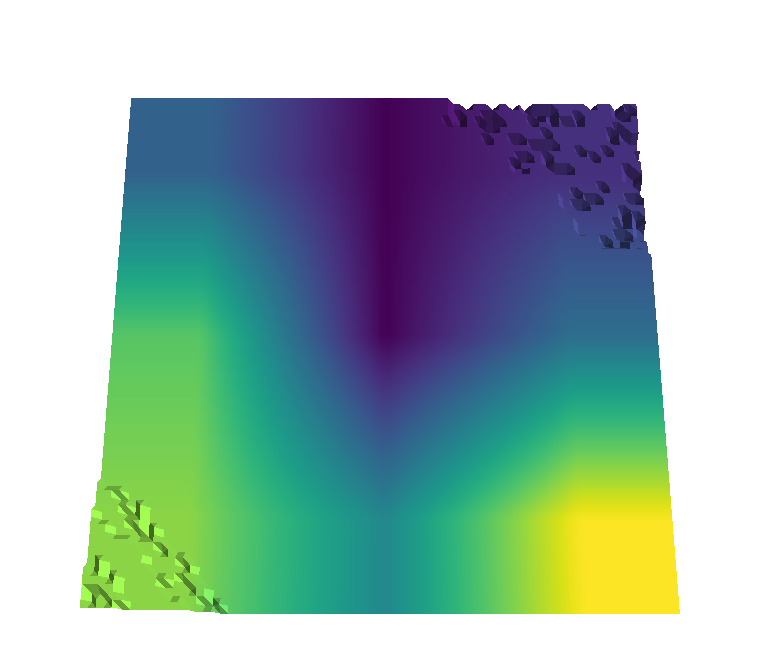
\includegraphics[width=\linewidth]{../img/5/quarry/best/25-patch-3d-majavi-colormap-10.png}
    \caption{0.26cm}
    \label{fig : quarry-best-1}
    \end{subfigure}
    \begin{subfigure}[b]{0.192\linewidth}
    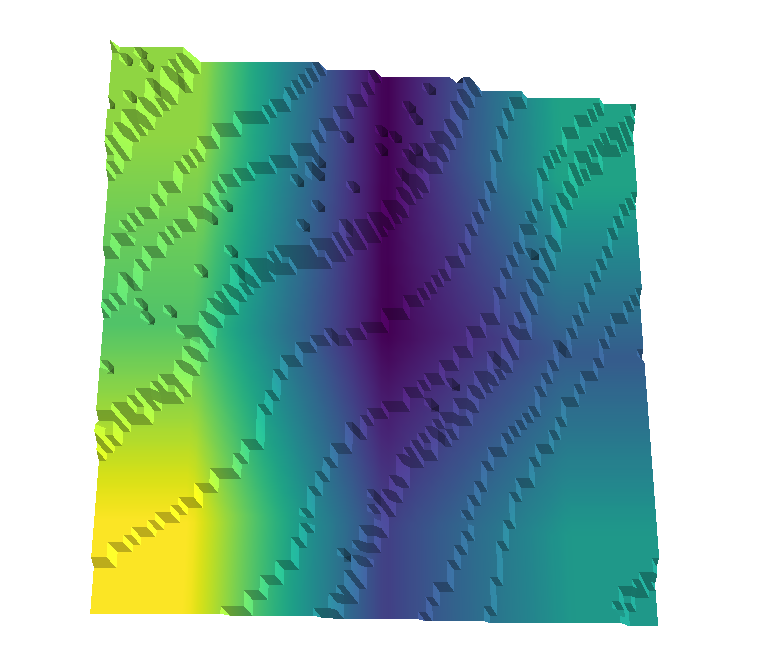
\includegraphics[width=\linewidth]{../img/5/quarry/best/30-patch-3d-majavi-colormap-20.png}
    \caption{0.30cm}
    \label{fig : quarry-best-2}
    \end{subfigure}
    \begin{subfigure}[b]{0.192\linewidth}
    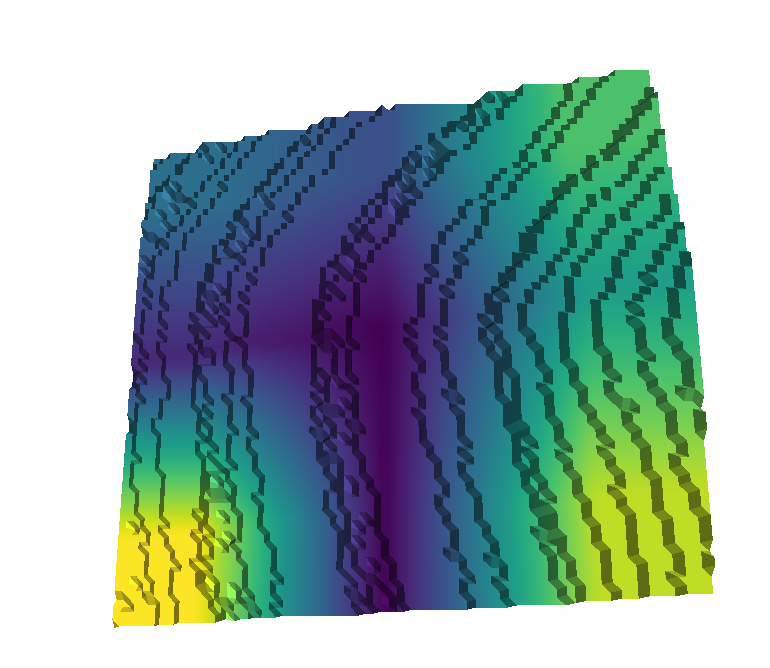
\includegraphics[width=\linewidth]{../img/5/quarry/best/34-patch-3d-majavi-colormap-30.png}
    \caption{0.35cm}
    \label{fig : quarry-best-3}
    \end{subfigure}
    \begin{subfigure}[b]{0.192\linewidth}
    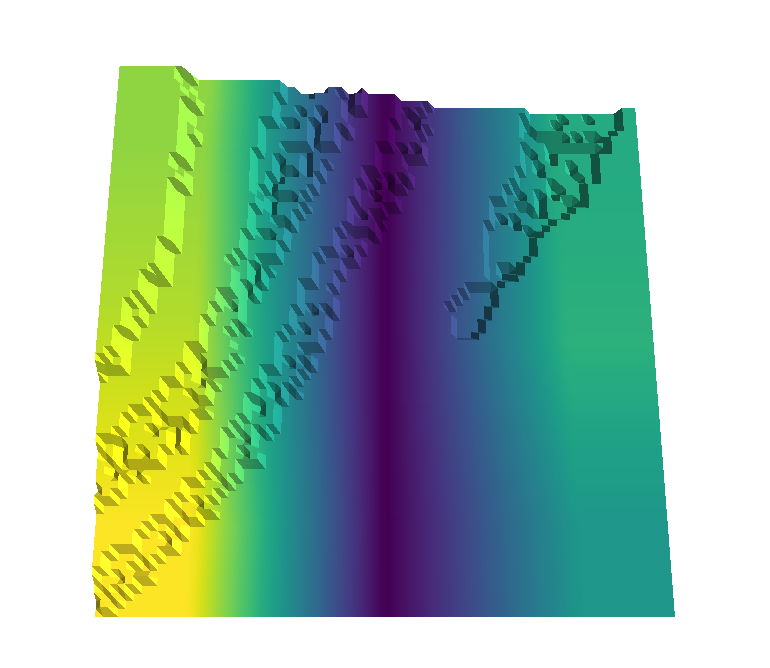
\includegraphics[width=\linewidth]{../img/5/quarry/best/38-patch-3d-majavi-colormap-40.png}
    \caption{0.38cm}
    \label{fig : quarry-best-4}
    \end{subfigure}
    \begin{subfigure}[b]{0.192\linewidth}
    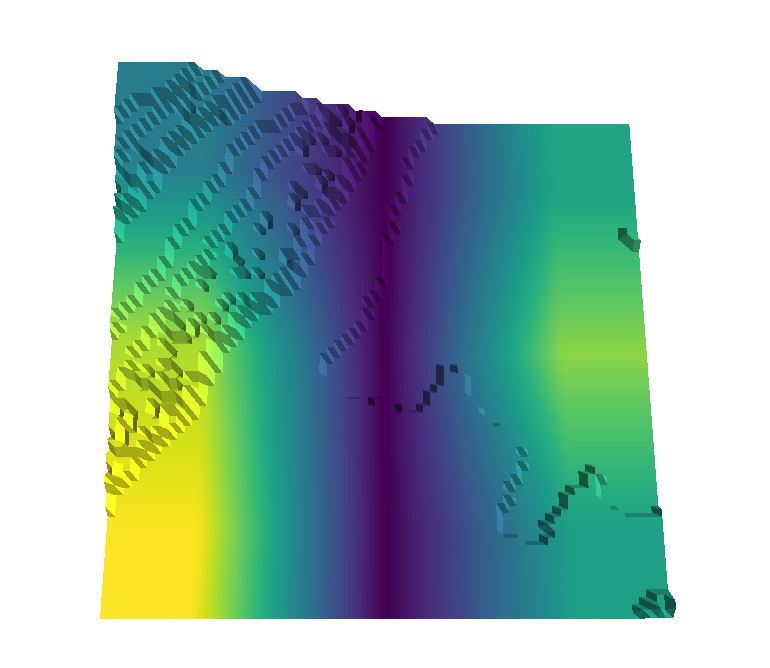
\includegraphics[width=\linewidth]{../img/5/quarry/best/41-patch-3d-majavi-colormap-50.png}
    \caption{0.41cm}
    \label{fig : quarry-best-5}
    \end{subfigure}
    \begin{subfigure}[b]{0.192\linewidth}
    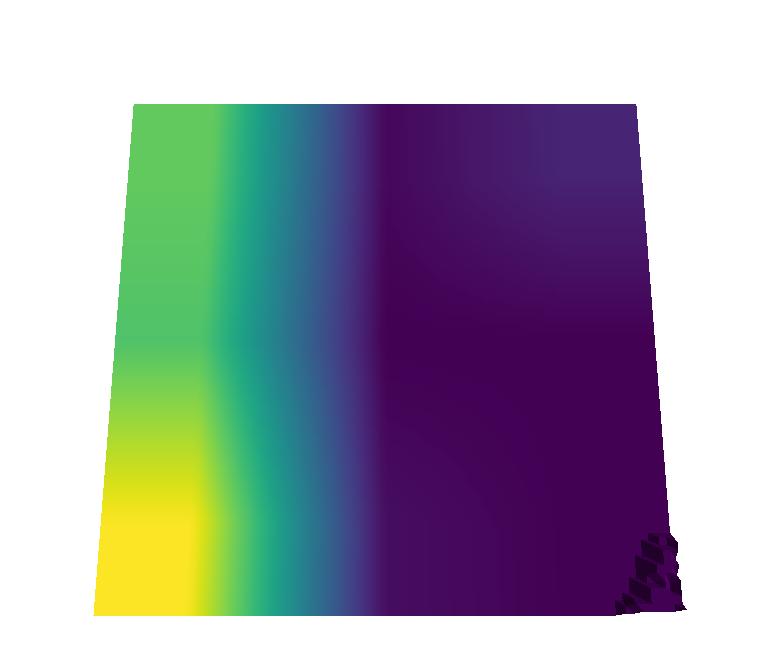
\includegraphics[width=\linewidth]{../img/5/quarry/best/44-patch-3d-majavi-colormap-60.png}
    \caption{0.44cm}
    \label{fig : quarry-best-6}
    \end{subfigure}
    \begin{subfigure}[b]{0.192\linewidth}
    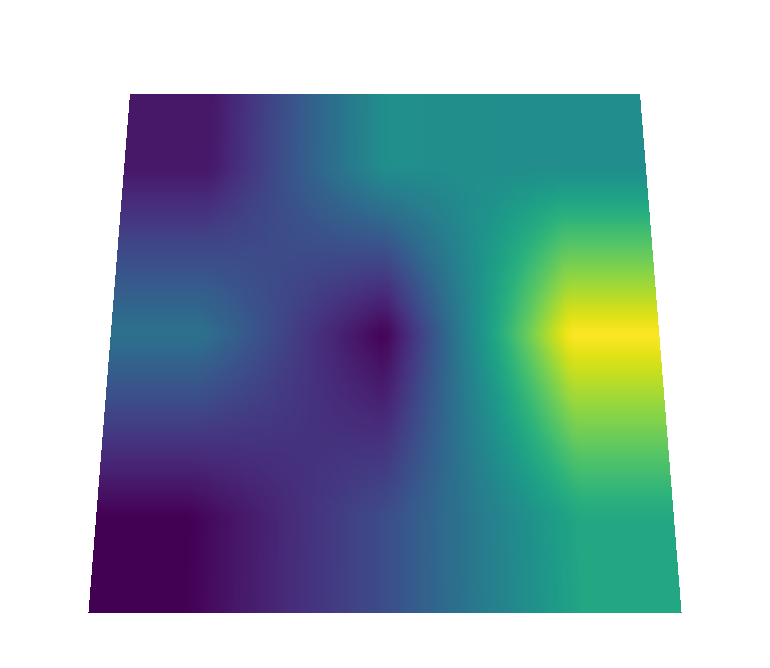
\includegraphics[width=\linewidth]{../img/5/quarry/best/46-patch-3d-majavi-colormap-70.png}
    \caption{0.47cm}
    \label{fig : quarry-best-7}
    \end{subfigure}
    \begin{subfigure}[b]{0.192\linewidth}
    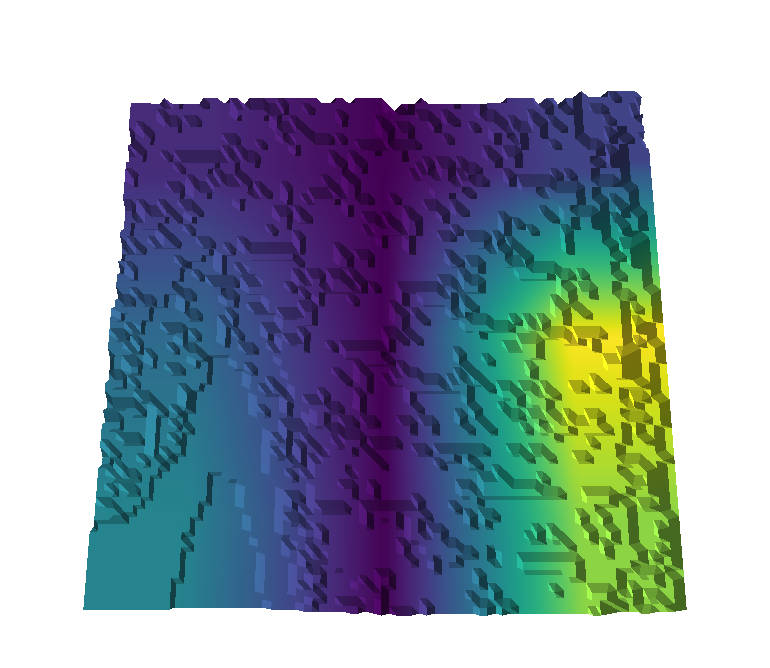
\includegraphics[width=\linewidth]{../img/5/quarry/best/49-patch-3d-majavi-colormap-80.png}
    \caption{0.49cm}
    \label{fig : quarry-best-8}
    \end{subfigure}
    \begin{subfigure}[b]{0.192\linewidth}
    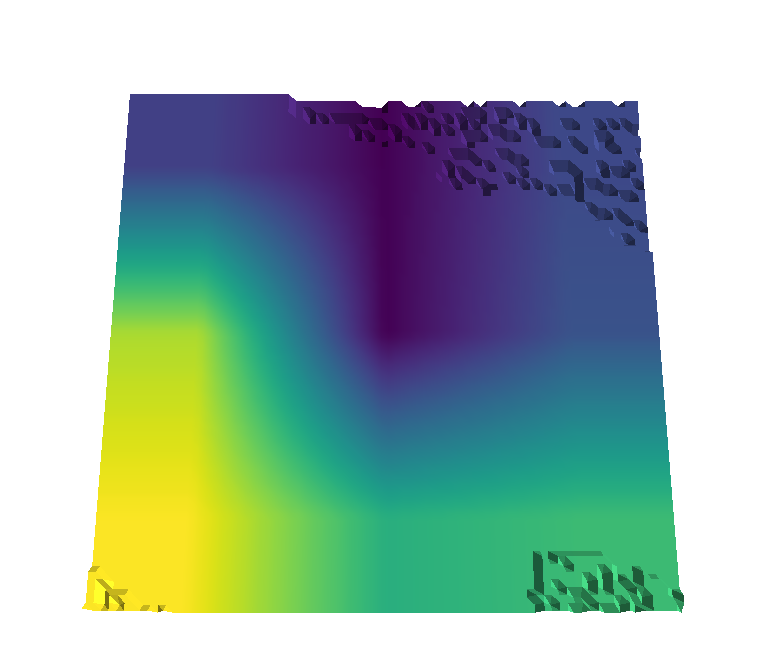
\includegraphics[width=\linewidth]{../img/5/quarry/best/51-patch-3d-majavi-colormap-90.png}
    \caption{0.52cm}
    \label{fig : quarry-best-9}
    \end{subfigure}
    \begin{subfigure}[b]{0.192\linewidth}
    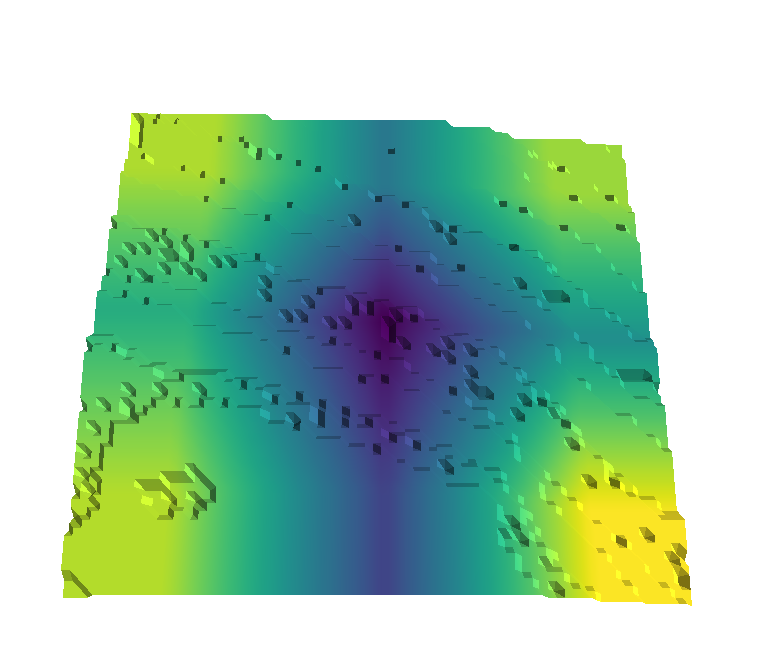
\includegraphics[width=\linewidth]{../img/5/quarry/best/54-patch-3d-majavi-colormap-100.png}
    \caption{0.54cm}
    \label{fig : quarry-best-10}
    \end{subfigure}
    \begin{subfigure}[b]{0.192\linewidth}
    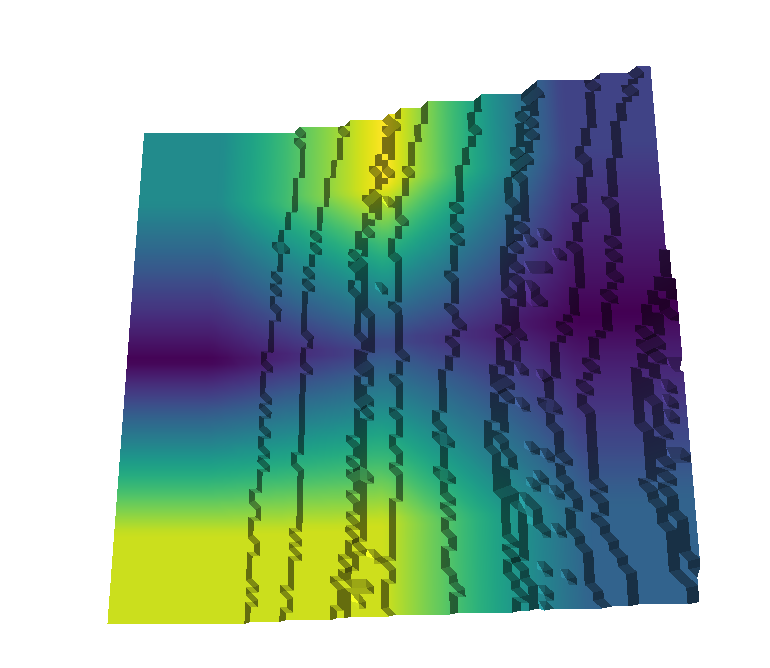
\includegraphics[width=\linewidth]{../img/5/quarry/best/56-patch-3d-majavi-colormap-110.png}
    \caption{0.57cm}
    \label{fig : quarry-best-11}
    \end{subfigure}
    \begin{subfigure}[b]{0.192\linewidth}
    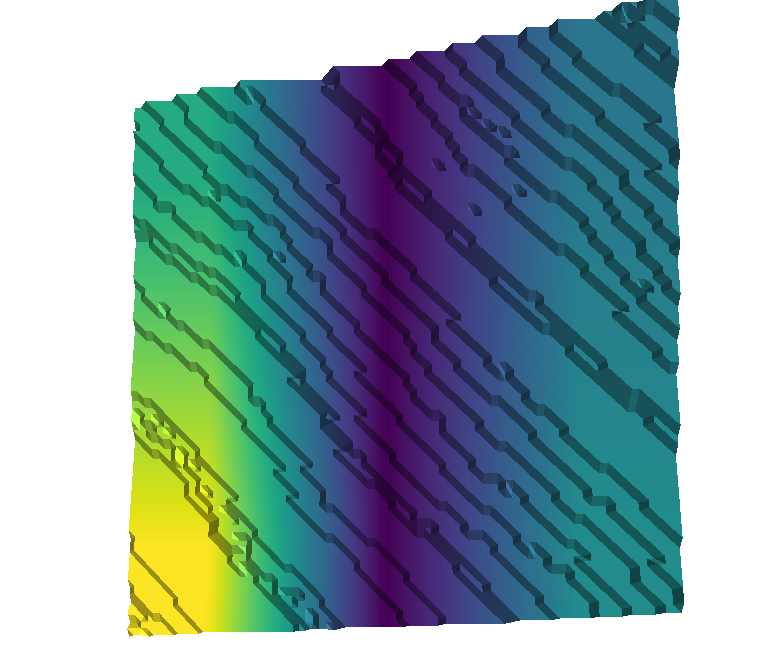
\includegraphics[width=\linewidth]{../img/5/quarry/best/58-patch-3d-majavi-colormap-120.png}
    \caption{0.59cm}
    \label{fig : quarry-best-12}
    \end{subfigure}
    \begin{subfigure}[b]{0.192\linewidth}
    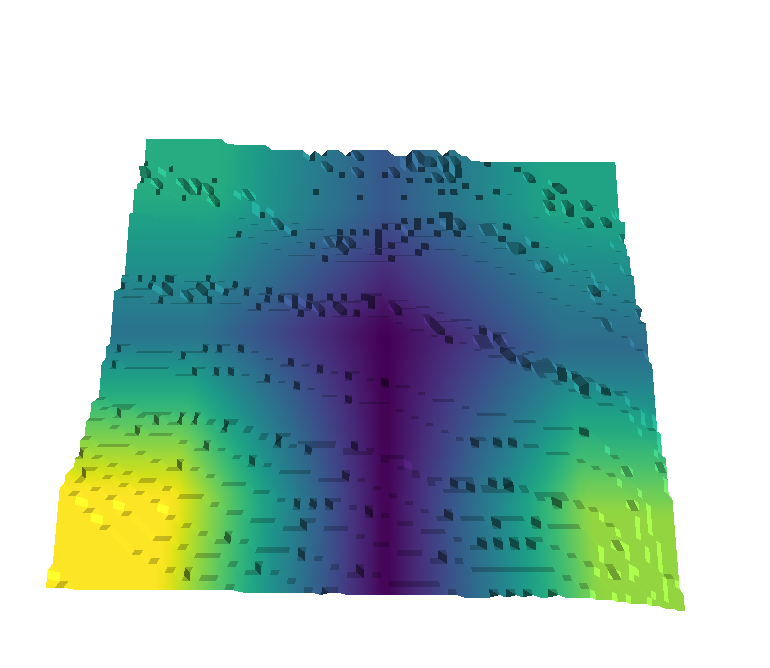
\includegraphics[width=\linewidth]{../img/5/quarry/best/60-patch-3d-majavi-colormap-130.png}
    \caption{0.60cm}
    \label{fig : quarry-best-13}
    \end{subfigure}
    \begin{subfigure}[b]{0.192\linewidth}
    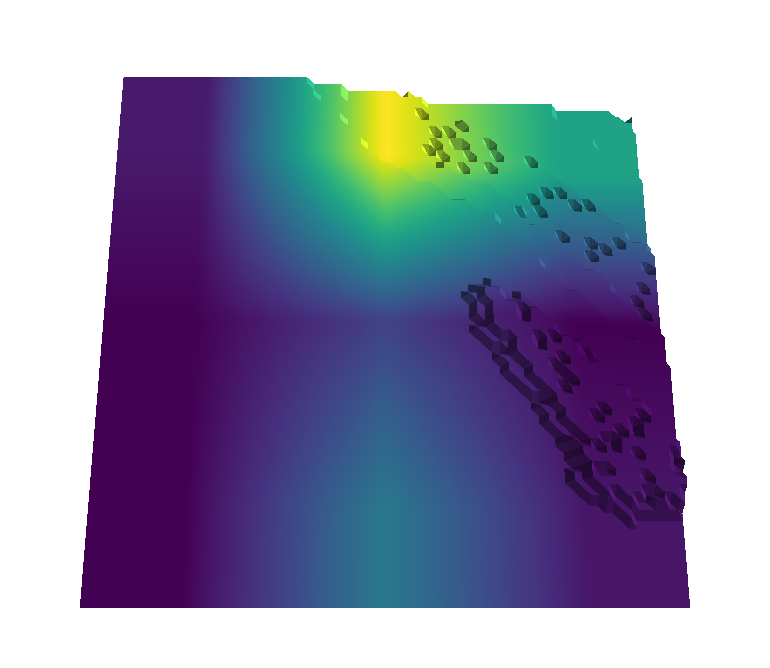
\includegraphics[width=\linewidth]{../img/5/quarry/best/62-patch-3d-majavi-colormap-140.png}
    \caption{0.62cm}
    \label{fig : quarry-best-14}
    \end{subfigure}
    \begin{subfigure}[b]{0.192\linewidth}
    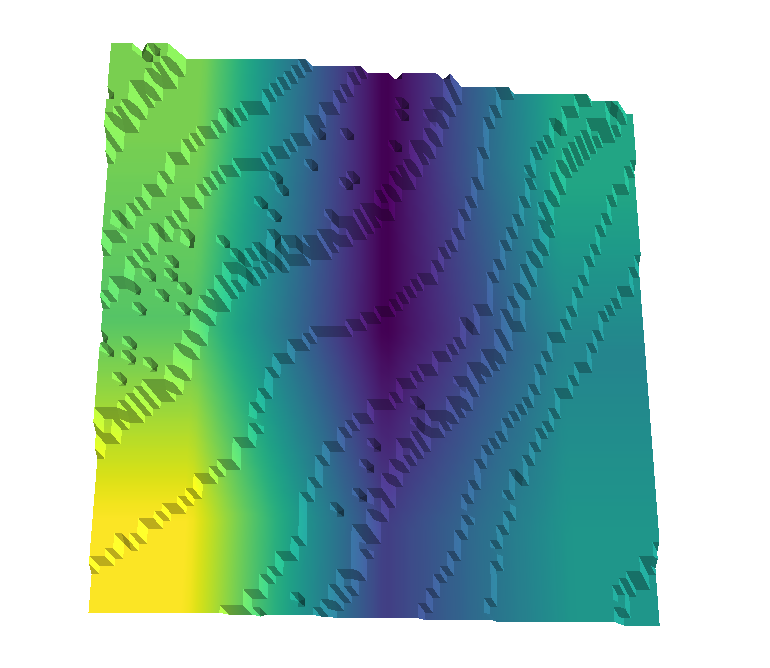
\includegraphics[width=\linewidth]{../img/5/quarry/best/63-patch-3d-majavi-colormap-150.png}
    \caption{0.64cm}
    \label{fig : quarry-best-15}
    \end{subfigure}
    \begin{subfigure}[b]{0.192\linewidth}
    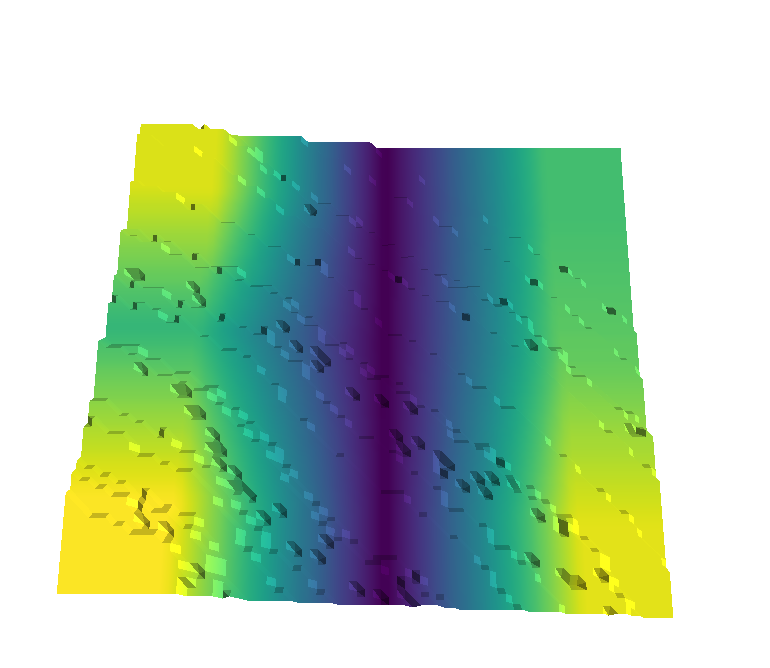
\includegraphics[width=\linewidth]{../img/5/quarry/best/65-patch-3d-majavi-colormap-160.png}
    \caption{0.66cm}
    \label{fig : quarry-best-16}
    \end{subfigure}
    \begin{subfigure}[b]{0.192\linewidth}
    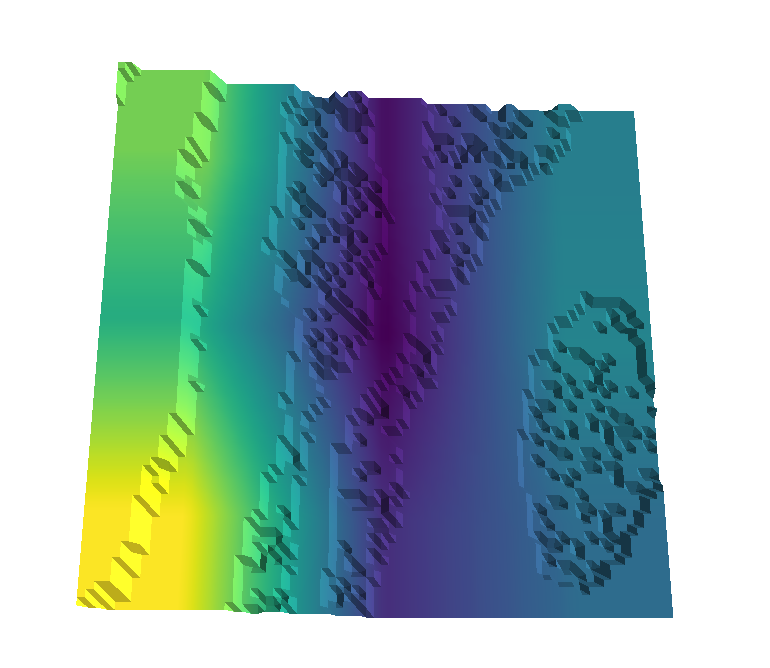
\includegraphics[width=\linewidth]{../img/5/quarry/best/67-patch-3d-majavi-colormap-170.png}
    \caption{0.67cm}
    \label{fig : quarry-best-17}
    \end{subfigure}
    \begin{subfigure}[b]{0.192\linewidth}
    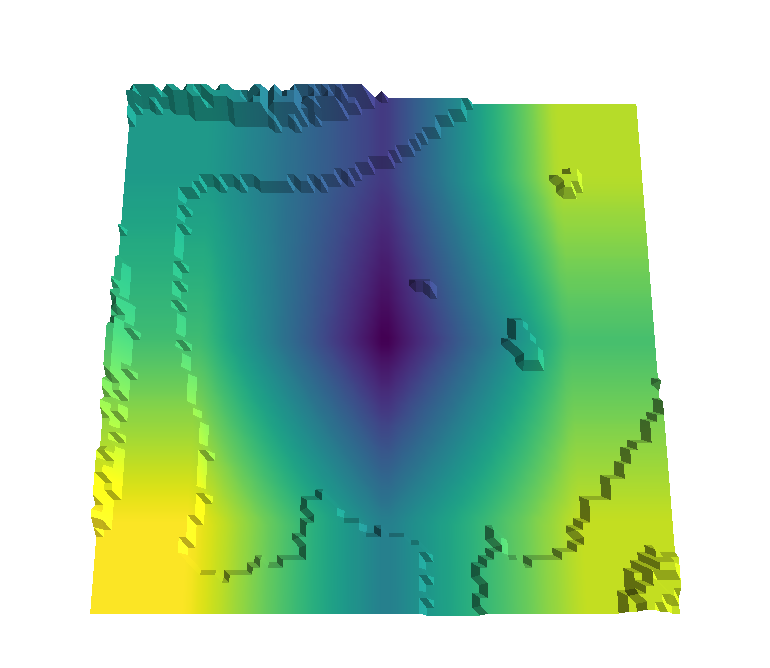
\includegraphics[width=\linewidth]{../img/5/quarry/best/68-patch-3d-majavi-colormap-180.png}
    \caption{0.68cm}
    \label{fig : quarry-best-18}
    \end{subfigure}
    \begin{subfigure}[b]{0.192\linewidth}
    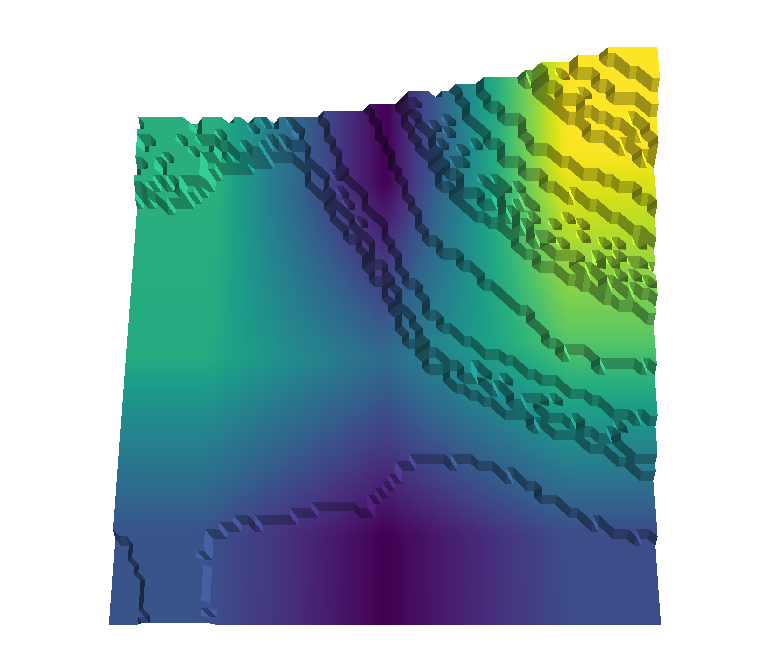
\includegraphics[width=\linewidth]{../img/5/quarry/best/70-patch-3d-majavi-colormap-190.png}
    \caption{0.70cm}
    \label{fig : quarry-best-19}
    \end{subfigure}
    \label{fig : quarry-best}
    \end{figure}

\subsection{Worst}
\begin{figure}[H]
    \centering
    \begin{subfigure}[b]{0.192\linewidth}
    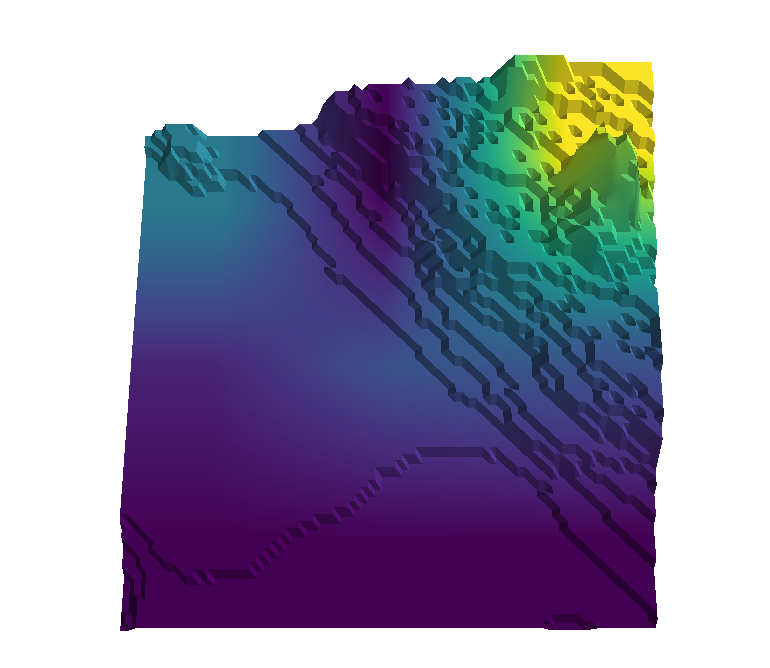
\includegraphics[width=\linewidth]{../img/5/quarry/worst/-35-patch-3d-majavi-colormap-0.png}
    \caption{-0.36cm}
    \end{subfigure}
    \begin{subfigure}[b]{0.192\linewidth}
    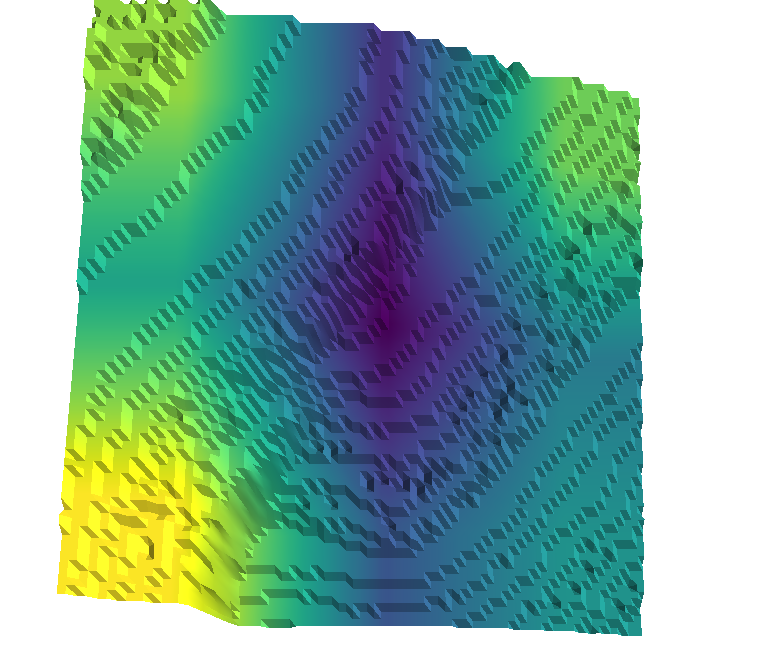
\includegraphics[width=\linewidth]{../img/5/quarry/worst/-7-patch-3d-majavi-colormap-10.png}
    \caption{-0.08cm}
    \end{subfigure}
    \begin{subfigure}[b]{0.192\linewidth}
    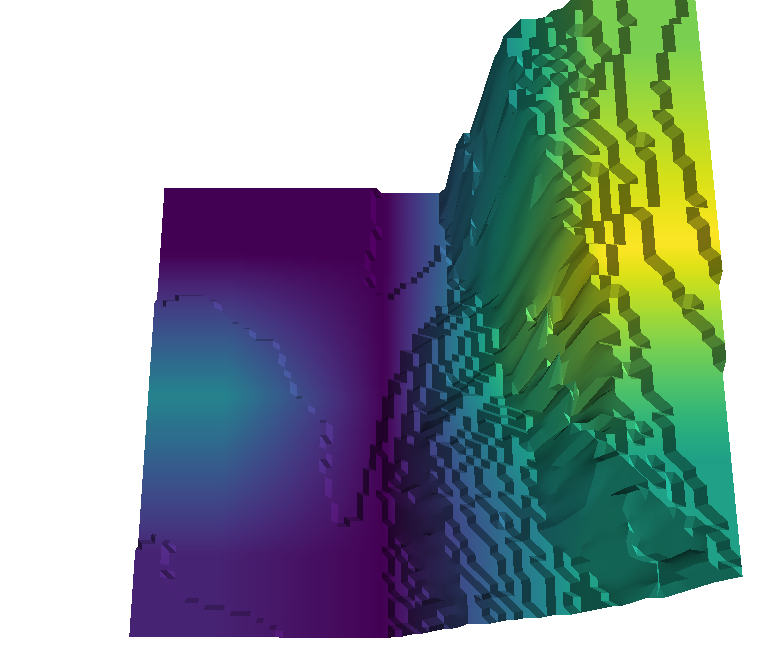
\includegraphics[width=\linewidth]{../img/5/quarry/worst/-4-patch-3d-majavi-colormap-20.png}
    \caption{-0.05cm}
    \end{subfigure}
    \begin{subfigure}[b]{0.192\linewidth}
    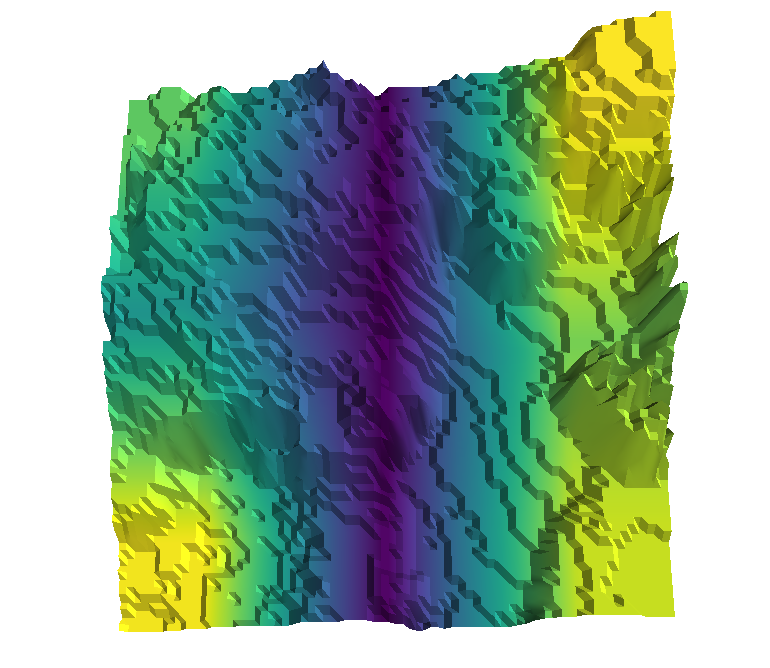
\includegraphics[width=\linewidth]{../img/5/quarry/worst/-3-patch-3d-majavi-colormap-30.png}
    \caption{-0.03cm}
    \end{subfigure}
    \begin{subfigure}[b]{0.192\linewidth}
    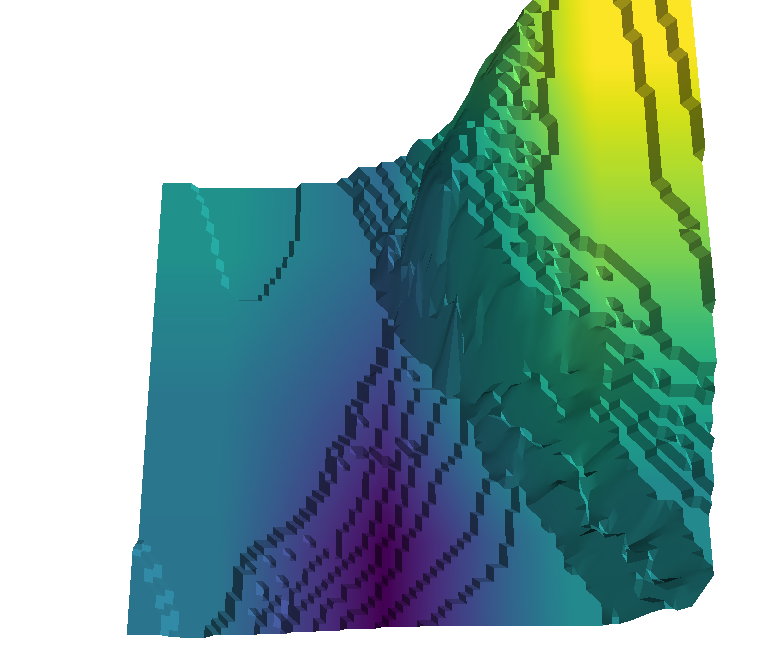
\includegraphics[width=\linewidth]{../img/5/quarry/worst/-2-patch-3d-majavi-colormap-40.png}
    \caption{-0.02cm}
    \end{subfigure}
    \begin{subfigure}[b]{0.192\linewidth}
    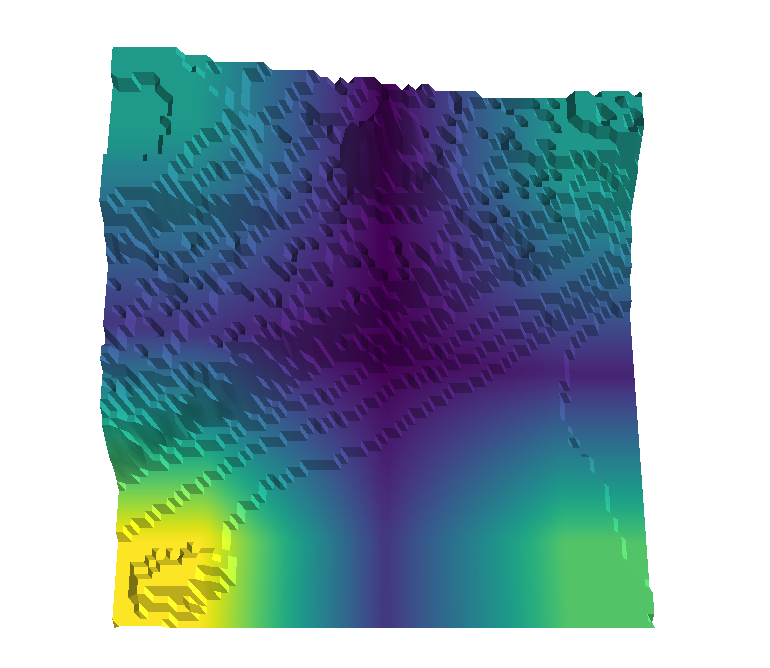
\includegraphics[width=\linewidth]{../img/5/quarry/worst/-1-patch-3d-majavi-colormap-50.png}
    \caption{-0.01cm}
    \end{subfigure}
    \begin{subfigure}[b]{0.192\linewidth}
    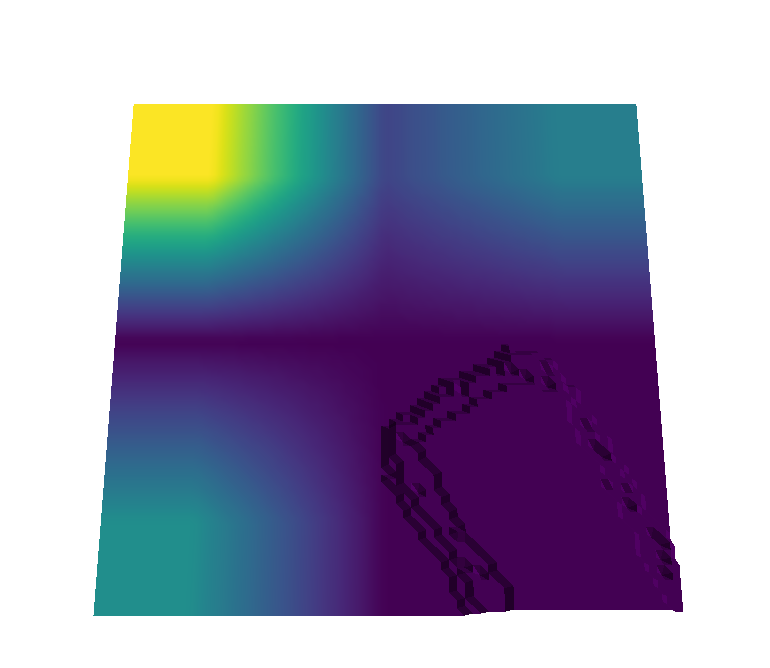
\includegraphics[width=\linewidth]{../img/5/quarry/worst/00-patch-3d-majavi-colormap-60.png}
    \caption{-0.01cm}
    \end{subfigure}
    \begin{subfigure}[b]{0.192\linewidth}
    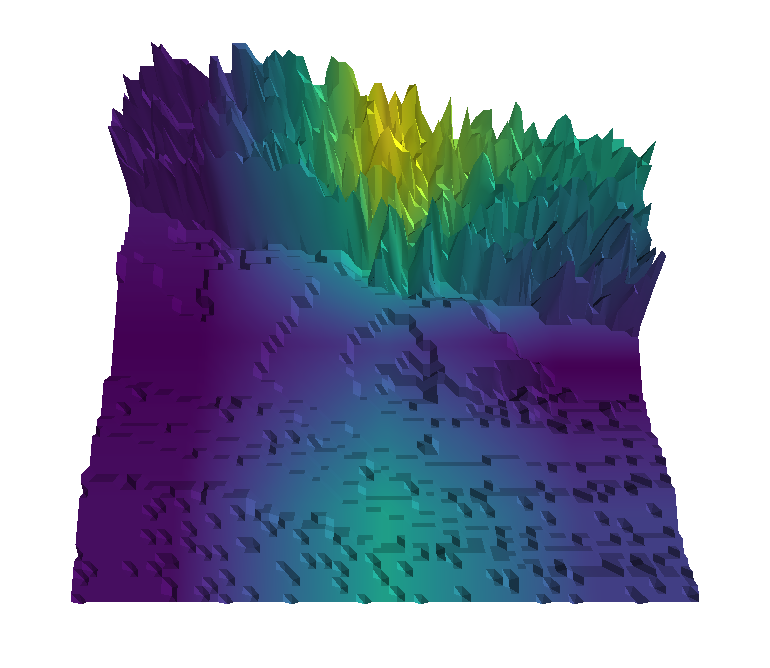
\includegraphics[width=\linewidth]{../img/5/quarry/worst/00-patch-3d-majavi-colormap-70.png}
    \caption{0.00cm}
    \end{subfigure}
    \begin{subfigure}[b]{0.192\linewidth}
    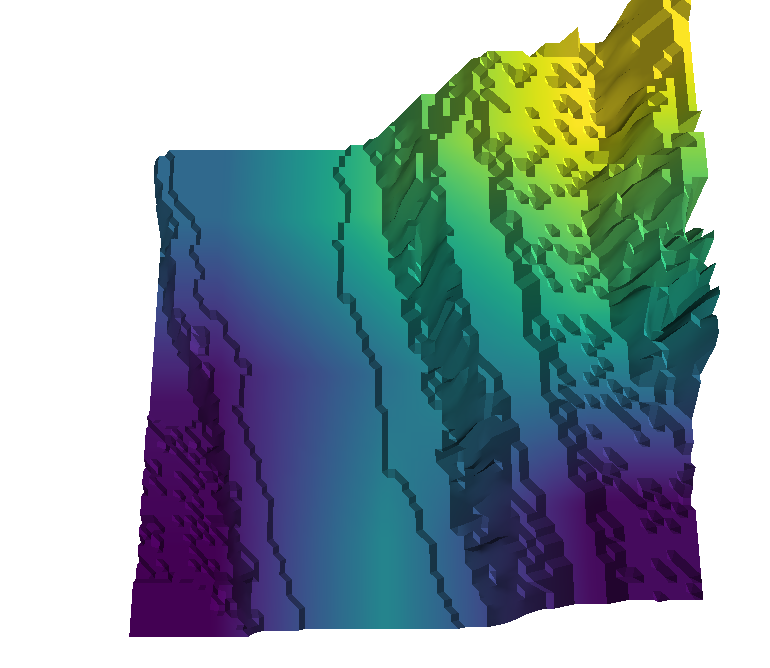
\includegraphics[width=\linewidth]{../img/5/quarry/worst/00-patch-3d-majavi-colormap-80.png}
    \caption{0.01cm}
    \end{subfigure}
    \begin{subfigure}[b]{0.192\linewidth}
    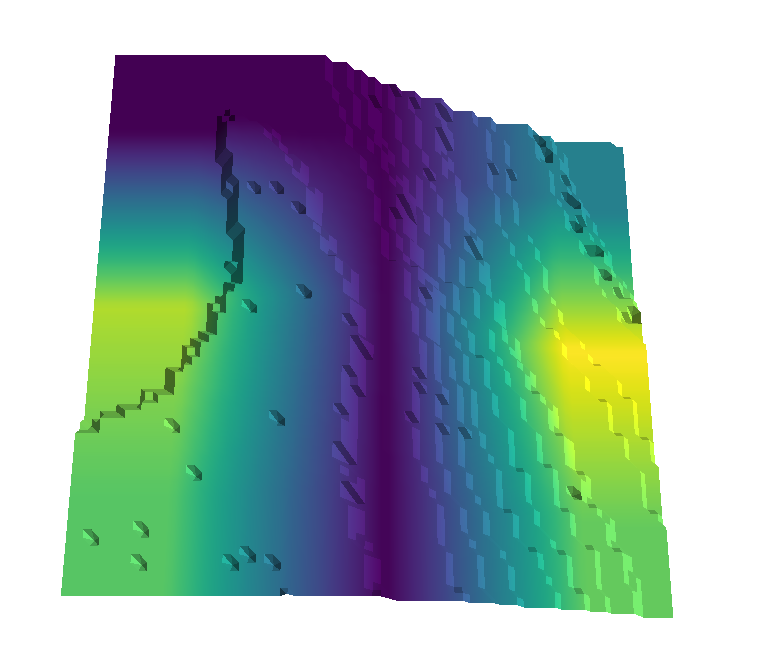
\includegraphics[width=\linewidth]{../img/5/quarry/worst/01-patch-3d-majavi-colormap-90.png}
    \caption{0.02cm}
    \end{subfigure}
    \begin{subfigure}[b]{0.192\linewidth}
    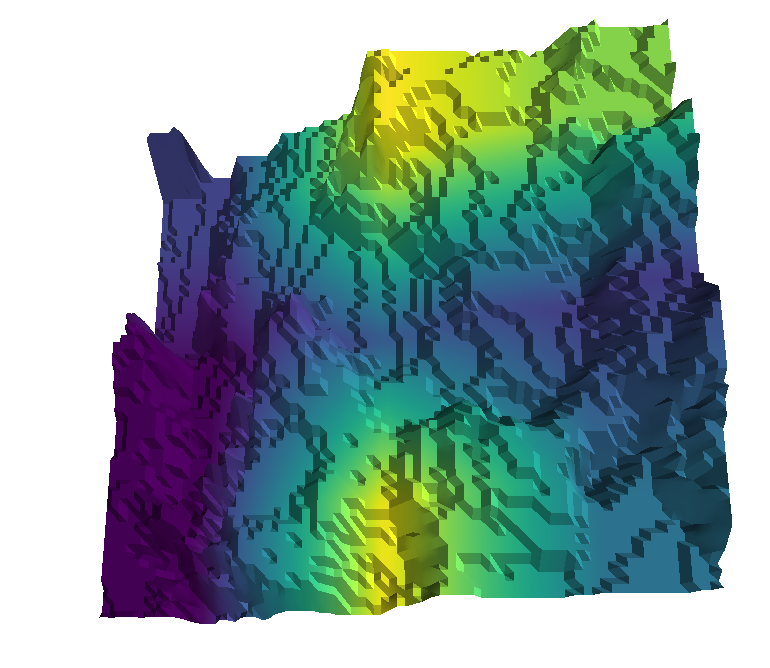
\includegraphics[width=\linewidth]{../img/5/quarry/worst/02-patch-3d-majavi-colormap-100.png}
    \caption{0.02cm}
    \end{subfigure}
    \begin{subfigure}[b]{0.192\linewidth}
    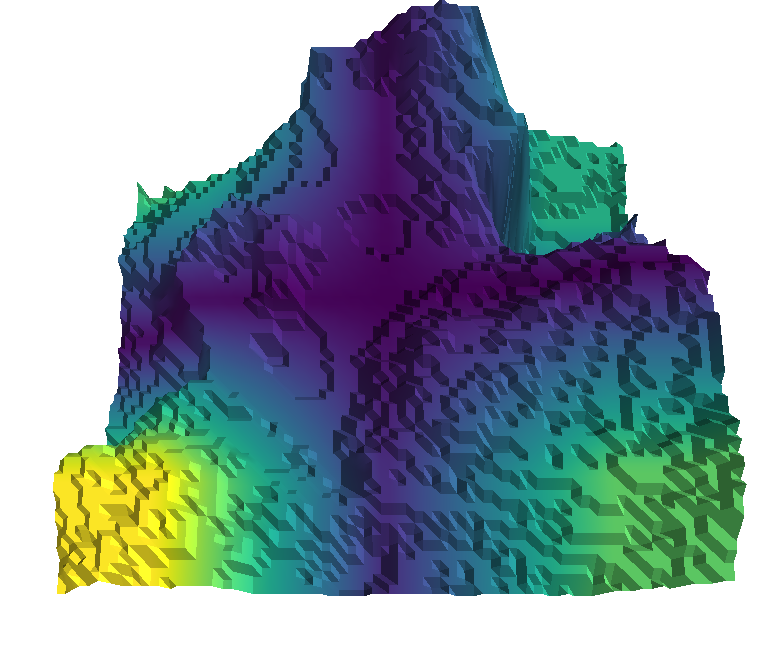
\includegraphics[width=\linewidth]{../img/5/quarry/worst/03-patch-3d-majavi-colormap-110.png}
    \caption{0.03cm}
    \end{subfigure}
    \begin{subfigure}[b]{0.192\linewidth}
    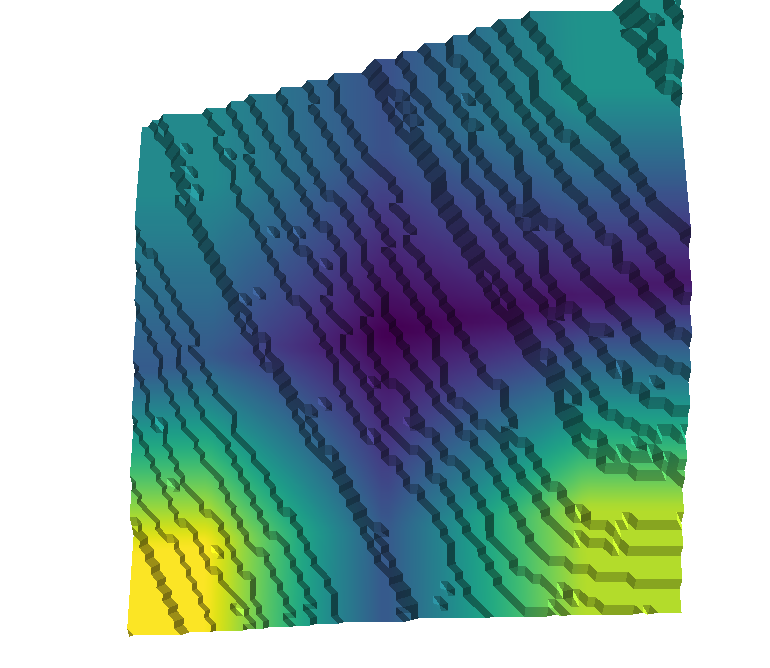
\includegraphics[width=\linewidth]{../img/5/quarry/worst/04-patch-3d-majavi-colormap-120.png}
    \caption{0.05cm}
    \end{subfigure}
    \begin{subfigure}[b]{0.192\linewidth}
    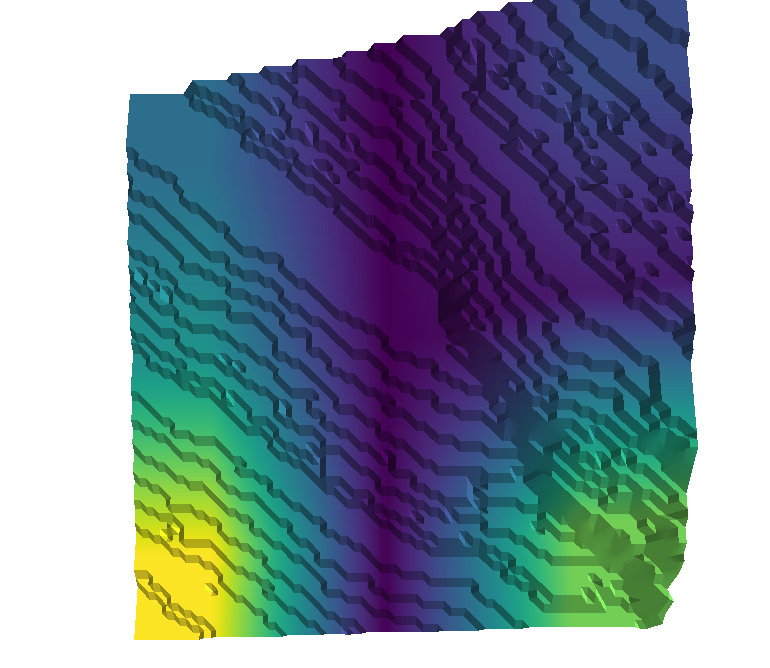
\includegraphics[width=\linewidth]{../img/5/quarry/worst/06-patch-3d-majavi-colormap-130.png}
    \caption{0.06cm}
    \end{subfigure}
    \begin{subfigure}[b]{0.192\linewidth}
    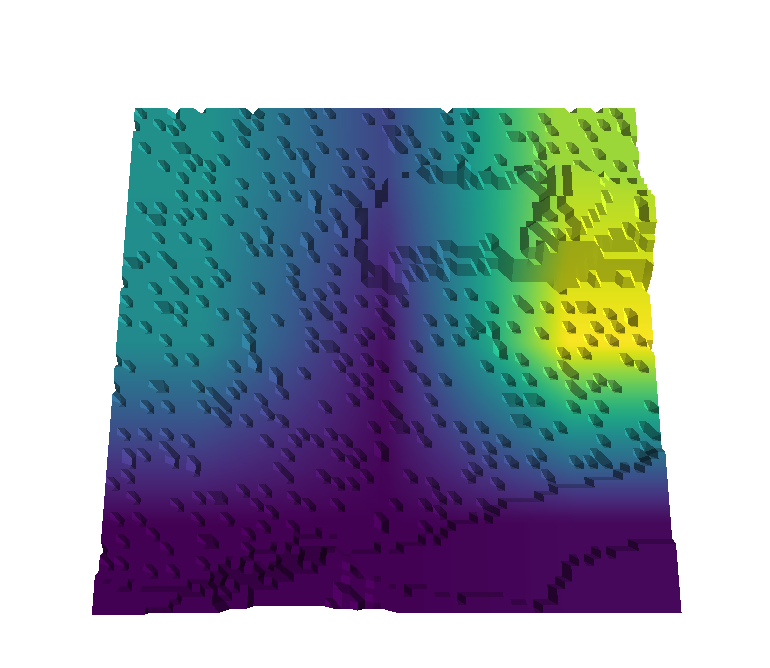
\includegraphics[width=\linewidth]{../img/5/quarry/worst/07-patch-3d-majavi-colormap-140.png}
    \caption{0.08cm}
    \end{subfigure}
    \begin{subfigure}[b]{0.192\linewidth}
    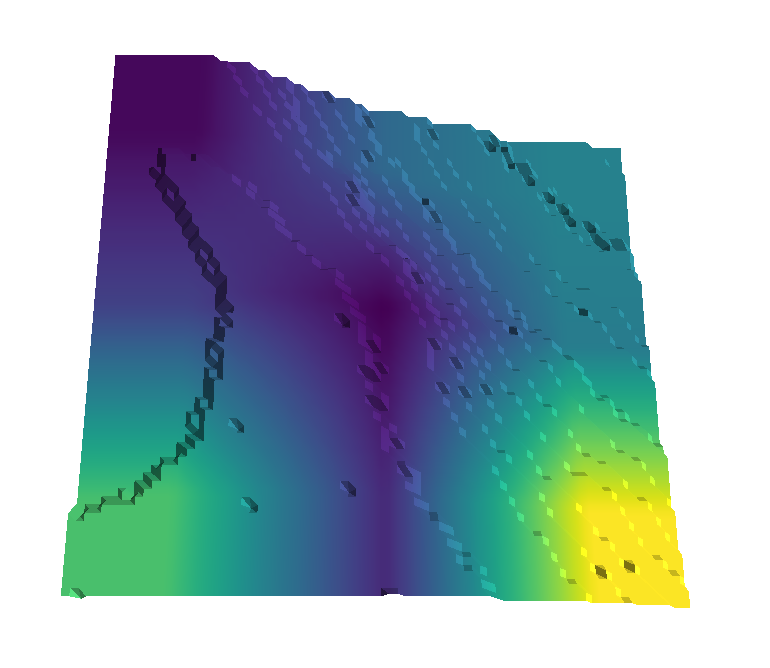
\includegraphics[width=\linewidth]{../img/5/quarry/worst/09-patch-3d-majavi-colormap-150.png}
    \caption{0.10cm}
    \end{subfigure}
    \begin{subfigure}[b]{0.192\linewidth}
    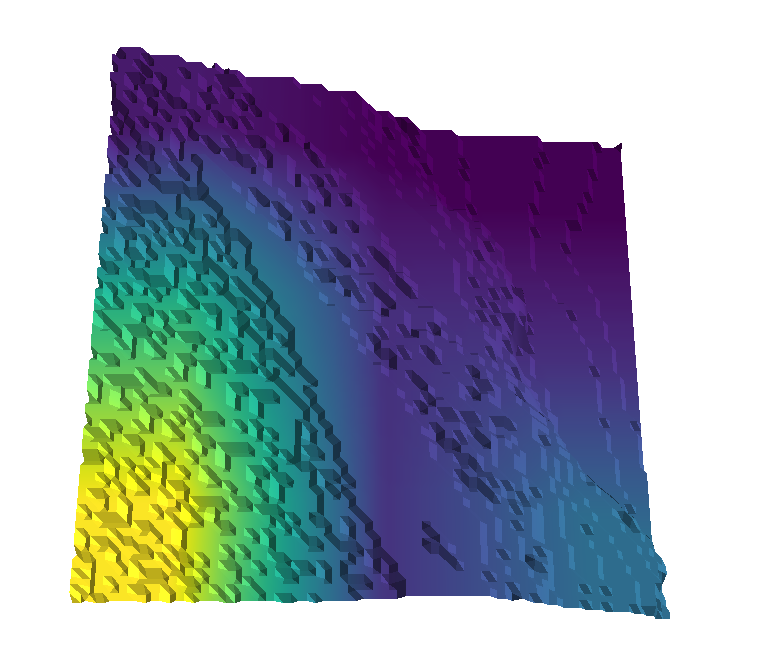
\includegraphics[width=\linewidth]{../img/5/quarry/worst/11-patch-3d-majavi-colormap-160.png}
    \caption{0.11cm}
    \end{subfigure}
    \begin{subfigure}[b]{0.192\linewidth}
    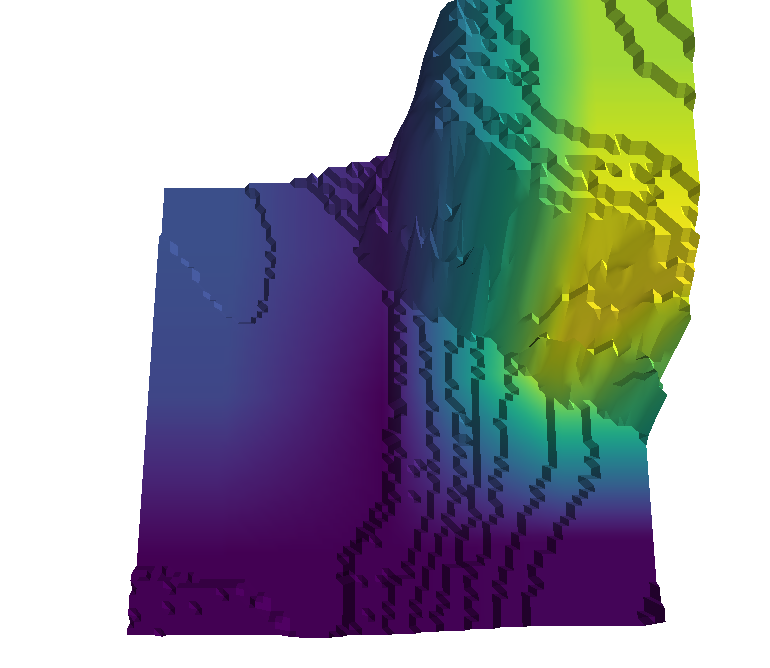
\includegraphics[width=\linewidth]{../img/5/quarry/worst/13-patch-3d-majavi-colormap-170.png}
    \caption{0.13cm}
    \end{subfigure}
    \begin{subfigure}[b]{0.192\linewidth}
    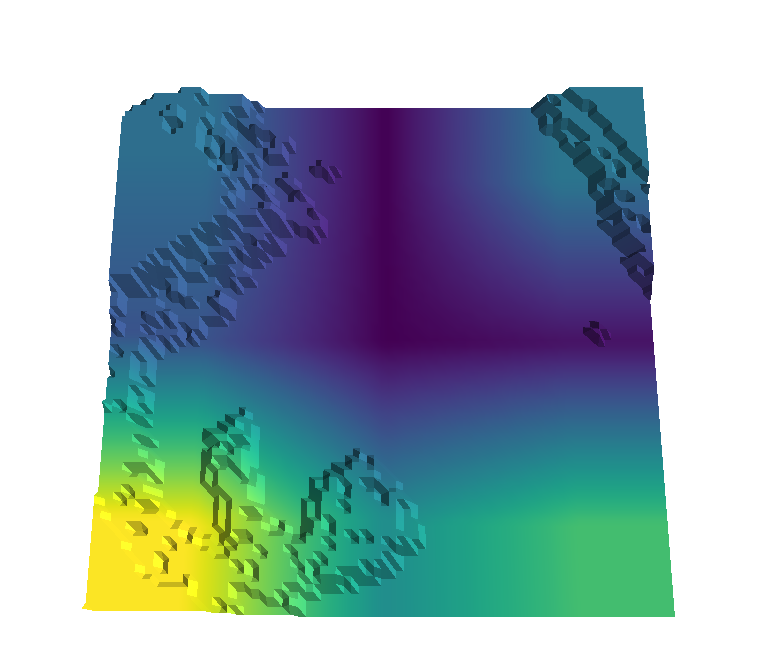
\includegraphics[width=\linewidth]{../img/5/quarry/worst/15-patch-3d-majavi-colormap-180.png}
    \caption{0.15cm}
    \end{subfigure}
    \begin{subfigure}[b]{0.192\linewidth}
    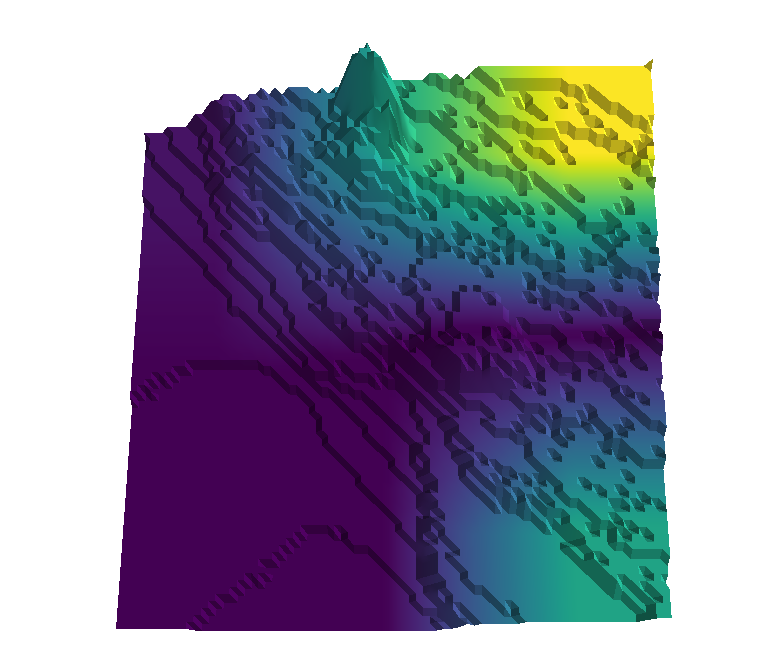
\includegraphics[width=\linewidth]{../img/5/quarry/worst/17-patch-3d-majavi-colormap-190.png}
    \caption{0.17cm}
    \end{subfigure}
    \begin{subfigure}[b]{0.192\linewidth}
    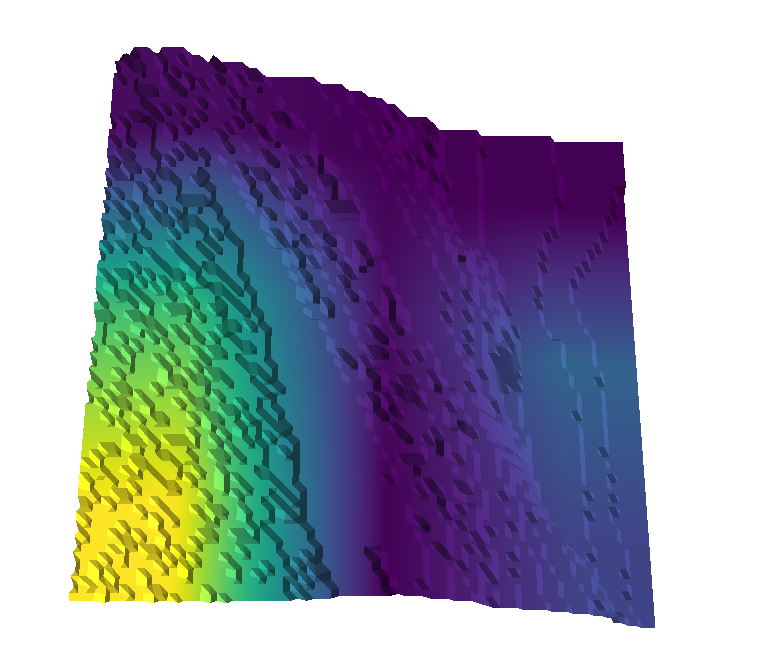
\includegraphics[width=\linewidth]{../img/5/quarry/worst/19-patch-3d-majavi-colormap-200.png}
    \caption{0.20cm}
    \end{subfigure}
    \end{figure}
\subsection{False Negative}
\begin{figure}[H]
    \centering
    \begin{subfigure}[b]{0.192\linewidth}
    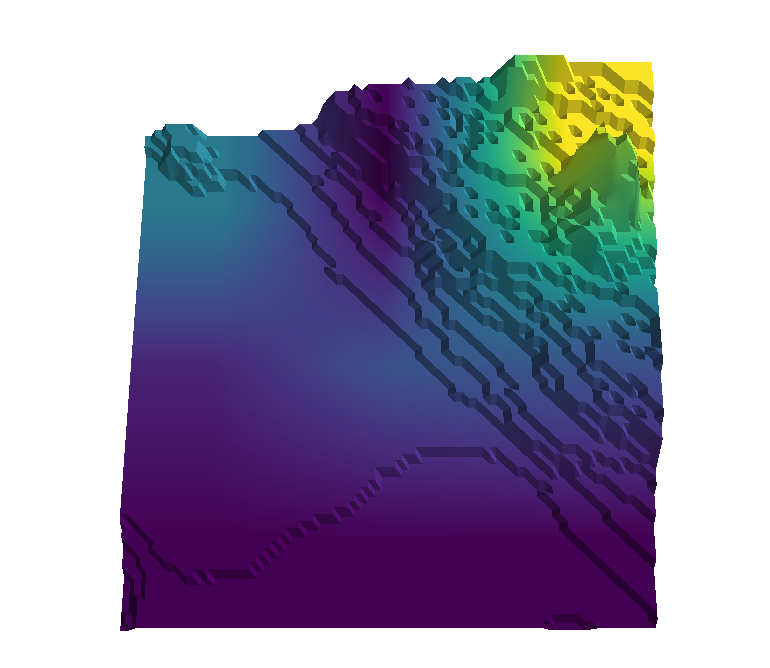
\includegraphics[width=\linewidth]{../img/5/quarry/false_negative/-14-patch-3d-majavi-colormap-0.png}
    \caption{-0.14cm}
    \end{subfigure}
    \begin{subfigure}[b]{0.192\linewidth}
    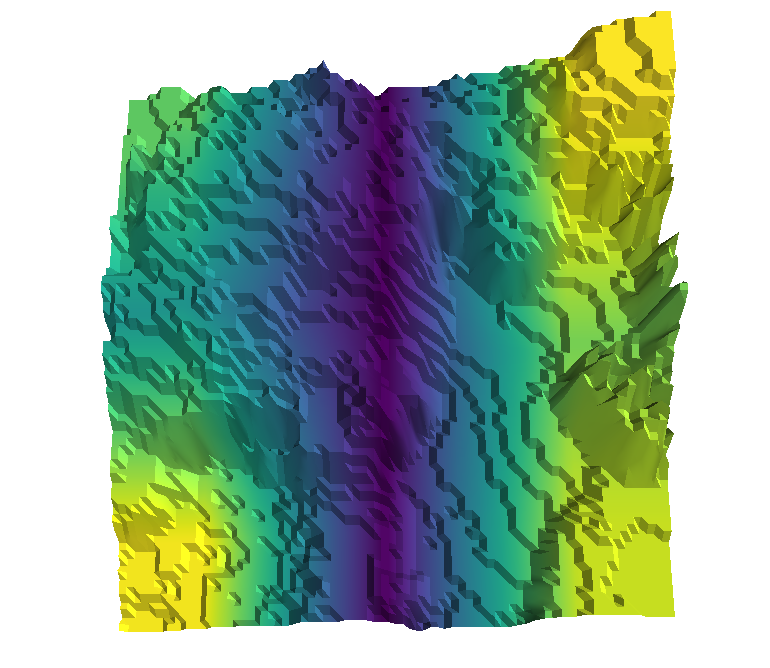
\includegraphics[width=\linewidth]{../img/5/quarry/false_negative/-6-patch-3d-majavi-colormap-10.png}
    \caption{-0.07cm}
    \end{subfigure}
    \begin{subfigure}[b]{0.192\linewidth}
    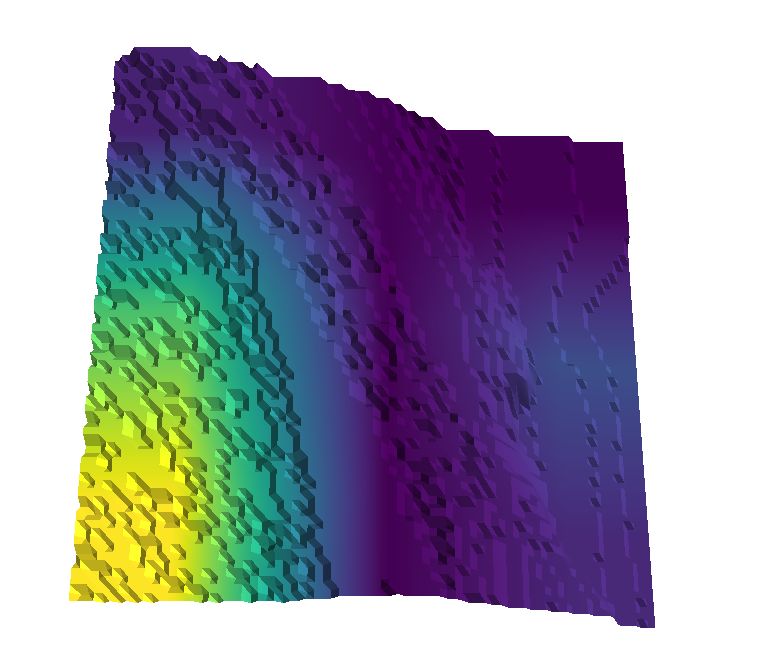
\includegraphics[width=\linewidth]{../img/5/quarry/false_negative/-4-patch-3d-majavi-colormap-20.png}
    \caption{-0.05cm}
    \end{subfigure}
    \begin{subfigure}[b]{0.192\linewidth}
    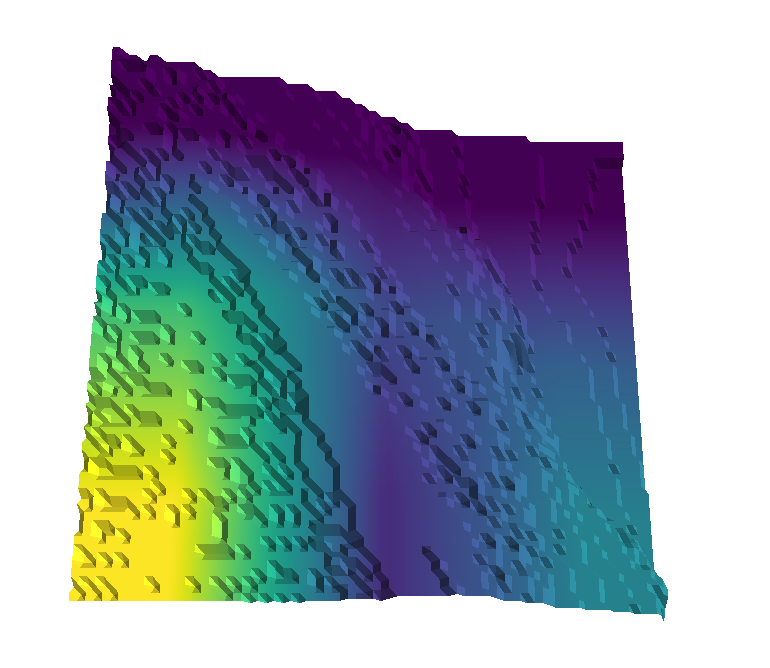
\includegraphics[width=\linewidth]{../img/5/quarry/false_negative/-2-patch-3d-majavi-colormap-30.png}
    \caption{-0.02cm}
    \end{subfigure}
    \begin{subfigure}[b]{0.192\linewidth}
    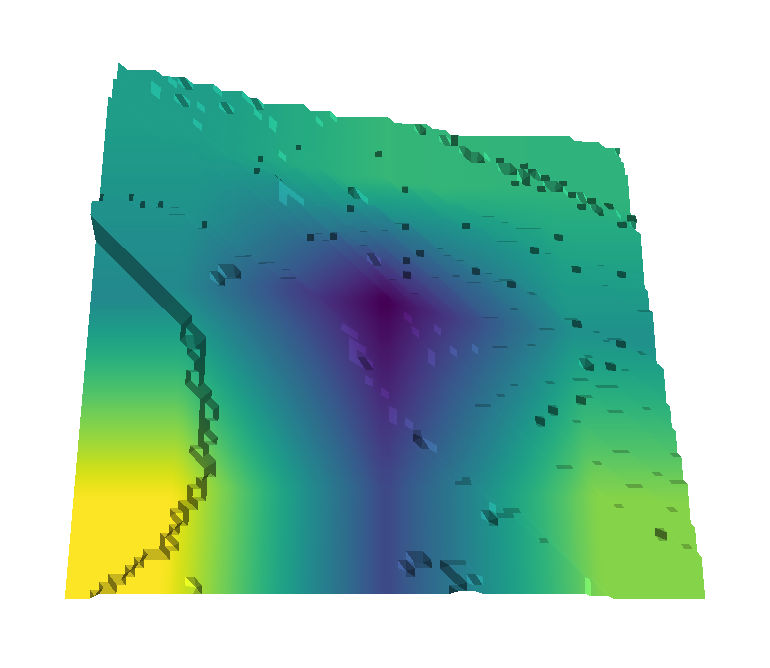
\includegraphics[width=\linewidth]{../img/5/quarry/false_negative/00-patch-3d-majavi-colormap-40.png}
    \caption{-0.00cm}
    \end{subfigure}
    \begin{subfigure}[b]{0.192\linewidth}
    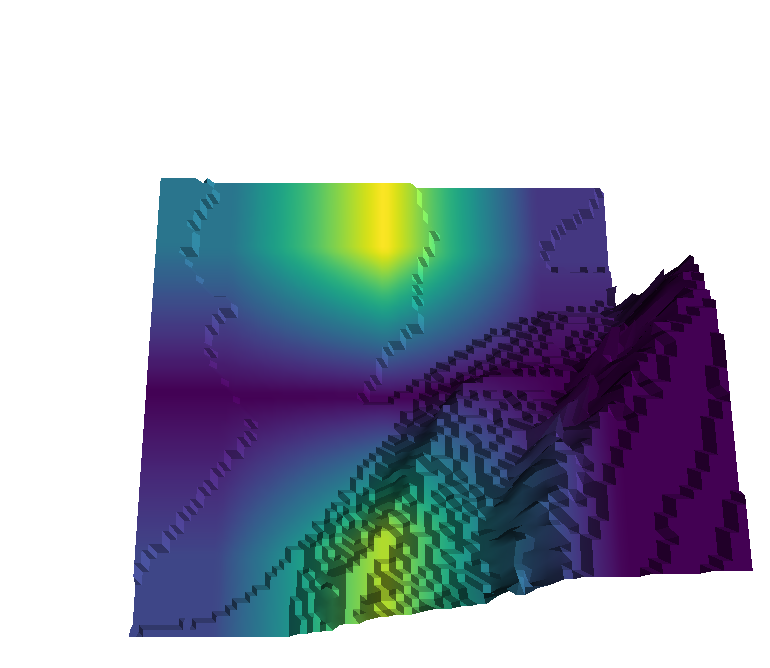
\includegraphics[width=\linewidth]{../img/5/quarry/false_negative/01-patch-3d-majavi-colormap-50.png}
    \caption{0.01cm}
    \end{subfigure}
    \begin{subfigure}[b]{0.192\linewidth}
    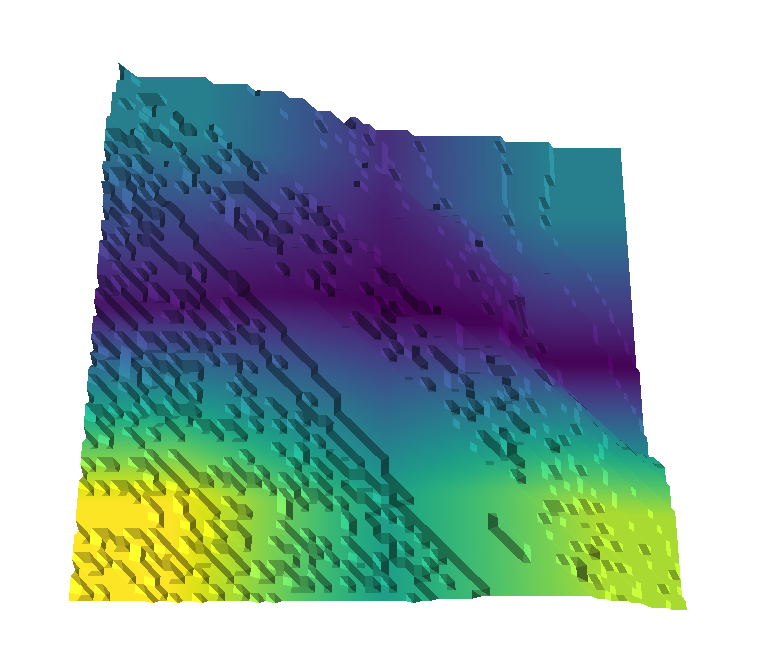
\includegraphics[width=\linewidth]{../img/5/quarry/false_negative/02-patch-3d-majavi-colormap-60.png}
    \caption{0.03cm}
    \end{subfigure}
    \begin{subfigure}[b]{0.192\linewidth}
    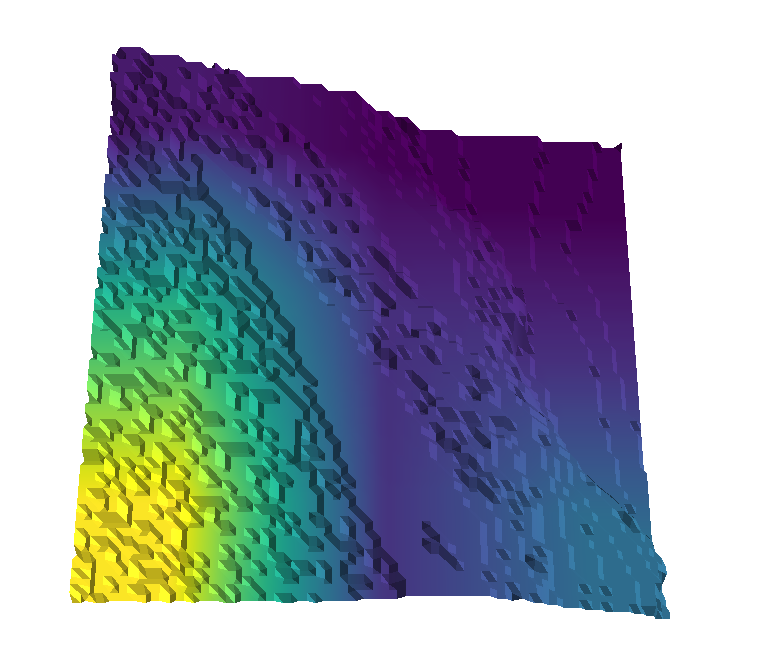
\includegraphics[width=\linewidth]{../img/5/quarry/false_negative/04-patch-3d-majavi-colormap-70.png}
    \caption{0.04cm}
    \end{subfigure}
    \begin{subfigure}[b]{0.192\linewidth}
    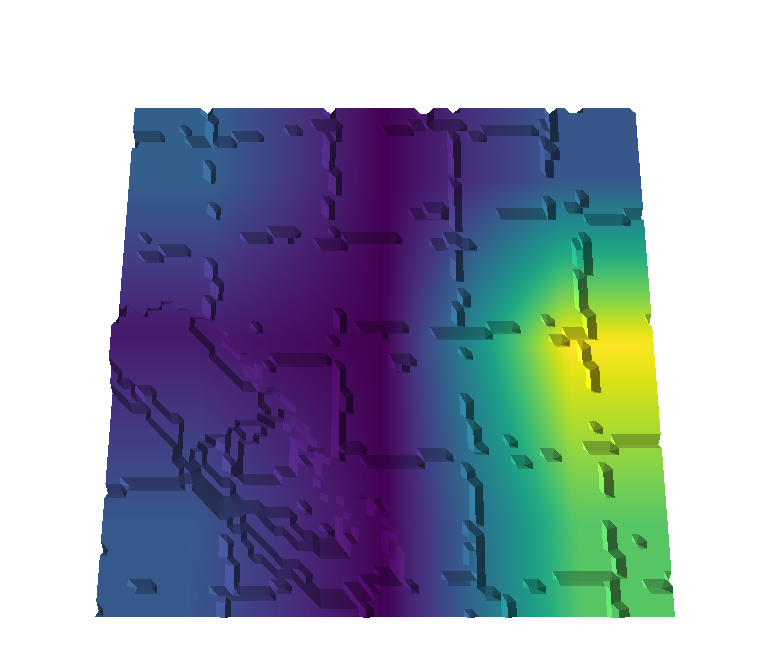
\includegraphics[width=\linewidth]{../img/5/quarry/false_negative/05-patch-3d-majavi-colormap-80.png}
    \caption{0.06cm}
    \end{subfigure}
    \begin{subfigure}[b]{0.192\linewidth}
    \includegraphics[width=\linewidth]{../img/5/quarry/false_negative/06-patch-3d-majavi-colormap-90.png}
    \caption{0.07cm}
    \end{subfigure}
    \begin{subfigure}[b]{0.192\linewidth}
    \includegraphics[width=\linewidth]{../img/5/quarry/false_negative/08-patch-3d-majavi-colormap-100.png}
    \caption{0.08cm}
    \end{subfigure}
    \begin{subfigure}[b]{0.192\linewidth}
    \includegraphics[width=\linewidth]{../img/5/quarry/false_negative/09-patch-3d-majavi-colormap-110.png}
    \caption{0.09cm}
    \end{subfigure}
    \begin{subfigure}[b]{0.192\linewidth}
    \includegraphics[width=\linewidth]{../img/5/quarry/false_negative/10-patch-3d-majavi-colormap-120.png}
    \caption{0.11cm}
    \end{subfigure}
    \begin{subfigure}[b]{0.192\linewidth}
    \includegraphics[width=\linewidth]{../img/5/quarry/false_negative/11-patch-3d-majavi-colormap-130.png}
    \caption{0.12cm}
    \end{subfigure}
    \begin{subfigure}[b]{0.192\linewidth}
    \includegraphics[width=\linewidth]{../img/5/quarry/false_negative/12-patch-3d-majavi-colormap-140.png}
    \caption{0.13cm}
    \end{subfigure}
    \begin{subfigure}[b]{0.192\linewidth}
    \includegraphics[width=\linewidth]{../img/5/quarry/false_negative/14-patch-3d-majavi-colormap-150.png}
    \caption{0.14cm}
    \end{subfigure}
    \begin{subfigure}[b]{0.192\linewidth}
    \includegraphics[width=\linewidth]{../img/5/quarry/false_negative/15-patch-3d-majavi-colormap-160.png}
    \caption{0.15cm}
    \end{subfigure}
    \begin{subfigure}[b]{0.192\linewidth}
    \includegraphics[width=\linewidth]{../img/5/quarry/false_negative/16-patch-3d-majavi-colormap-170.png}
    \caption{0.17cm}
    \end{subfigure}
    \begin{subfigure}[b]{0.192\linewidth}
    \includegraphics[width=\linewidth]{../img/5/quarry/false_negative/17-patch-3d-majavi-colormap-180.png}
    \caption{0.18cm}
    \end{subfigure}
    \begin{subfigure}[b]{0.192\linewidth}
    \includegraphics[width=\linewidth]{../img/5/quarry/false_negative/18-patch-3d-majavi-colormap-190.png}
    \caption{0.18cm}
    \end{subfigure}
    \begin{subfigure}[b]{0.192\linewidth}
    \includegraphics[width=\linewidth]{../img/5/quarry/false_negative/19-patch-3d-majavi-colormap-200.png}
    \caption{0.19cm}
    \end{subfigure}
    \end{figure}
\subsection{False Positive}
\begin{figure}[H]
    \centering
    \begin{subfigure}[b]{0.192\linewidth}
    \includegraphics[width=\linewidth]{../img/5/quarry/false_positive/20-patch-3d-majavi-colormap-0.png}
    \caption{0.20cm}
    \end{subfigure}
    \begin{subfigure}[b]{0.192\linewidth}
    \includegraphics[width=\linewidth]{../img/5/quarry/false_positive/20-patch-3d-majavi-colormap-12.png}
    \caption{0.21cm}
    \end{subfigure}
    \begin{subfigure}[b]{0.192\linewidth}
    \includegraphics[width=\linewidth]{../img/5/quarry/false_positive/22-patch-3d-majavi-colormap-24.png}
    \caption{0.22cm}
    \end{subfigure}
    \begin{subfigure}[b]{0.192\linewidth}
    \includegraphics[width=\linewidth]{../img/5/quarry/false_positive/23-patch-3d-majavi-colormap-36.png}
    \caption{0.23cm}
    \end{subfigure}
    \begin{subfigure}[b]{0.192\linewidth}
    \includegraphics[width=\linewidth]{../img/5/quarry/false_positive/24-patch-3d-majavi-colormap-48.png}
    \caption{0.24cm}
    \end{subfigure}
    \begin{subfigure}[b]{0.192\linewidth}
    \includegraphics[width=\linewidth]{../img/5/quarry/false_positive/25-patch-3d-majavi-colormap-60.png}
    \caption{0.25cm}
    \end{subfigure}
    \begin{subfigure}[b]{0.192\linewidth}
    \includegraphics[width=\linewidth]{../img/5/quarry/false_positive/25-patch-3d-majavi-colormap-72.png}
    \caption{0.26cm}
    \end{subfigure}
    \begin{subfigure}[b]{0.192\linewidth}
    \includegraphics[width=\linewidth]{../img/5/quarry/false_positive/26-patch-3d-majavi-colormap-84.png}
    \caption{0.27cm}
    \end{subfigure}
    \begin{subfigure}[b]{0.192\linewidth}
    \includegraphics[width=\linewidth]{../img/5/quarry/false_positive/27-patch-3d-majavi-colormap-96.png}
    \caption{0.27cm}
    \end{subfigure}
    \begin{subfigure}[b]{0.192\linewidth}
    \includegraphics[width=\linewidth]{../img/5/quarry/false_positive/27-patch-3d-majavi-colormap-108.png}
    \caption{0.28cm}
    \end{subfigure}
    \begin{subfigure}[b]{0.192\linewidth}
    \includegraphics[width=\linewidth]{../img/5/quarry/false_positive/29-patch-3d-majavi-colormap-120.png}
    \caption{0.29cm}
    \end{subfigure}
    \begin{subfigure}[b]{0.192\linewidth}
    \includegraphics[width=\linewidth]{../img/5/quarry/false_positive/30-patch-3d-majavi-colormap-132.png}
    \caption{0.30cm}
    \end{subfigure}
    \begin{subfigure}[b]{0.192\linewidth}
    \includegraphics[width=\linewidth]{../img/5/quarry/false_positive/31-patch-3d-majavi-colormap-144.png}
    \caption{0.32cm}
    \end{subfigure}
    \begin{subfigure}[b]{0.192\linewidth}
    \includegraphics[width=\linewidth]{../img/5/quarry/false_positive/33-patch-3d-majavi-colormap-156.png}
    \caption{0.34cm}
    \end{subfigure}
    \begin{subfigure}[b]{0.192\linewidth}
    \includegraphics[width=\linewidth]{../img/5/quarry/false_positive/35-patch-3d-majavi-colormap-168.png}
    \caption{0.35cm}
    \end{subfigure}
    \begin{subfigure}[b]{0.192\linewidth}
    \includegraphics[width=\linewidth]{../img/5/quarry/false_positive/36-patch-3d-majavi-colormap-180.png}
    \caption{0.36cm}
    \end{subfigure}
    \begin{subfigure}[b]{0.192\linewidth}
    \includegraphics[width=\linewidth]{../img/5/quarry/false_positive/38-patch-3d-majavi-colormap-192.png}
    \caption{0.39cm}
    \end{subfigure}
    \begin{subfigure}[b]{0.192\linewidth}
    \includegraphics[width=\linewidth]{../img/5/quarry/false_positive/41-patch-3d-majavi-colormap-204.png}
    \caption{0.41cm}
    \end{subfigure}
    \begin{subfigure}[b]{0.192\linewidth}
    \includegraphics[width=\linewidth]{../img/5/quarry/false_positive/46-patch-3d-majavi-colormap-216.png}
    \caption{0.46cm}
    \end{subfigure}
    \begin{subfigure}[b]{0.192\linewidth}
    \includegraphics[width=\linewidth]{../img/5/quarry/false_positive/51-patch-3d-majavi-colormap-228.png}
    \caption{0.52cm}
    \end{subfigure}
    \begin{subfigure}[b]{0.192\linewidth}
    \includegraphics[width=\linewidth]{../img/5/quarry/false_positive/61-patch-3d-majavi-colormap-240.png}
    \caption{0.62cm}
    \end{subfigure}
    \end{figure}

\end{document}